\chapter{Analysis}

In this chapter, I shortly introduce the reader to Memsource Cloud and its features, and move onto the requirements for the mobile application. Next, I cover the market shares of Android, iOS and Windows Phone, followed by an analysis of today's major cross-platform mobile app development tools. I discuss their features and conclude by picking React Native as the library of choice. 

\section{Working with Memsource Cloud}

Each of the target groups has a partially different way of working with the Memsource platform. Here, I will cover a usual workflow of a translation agency. Such agency typically has two main types of employees---project managers and translators (linguists). Project managers communicate with customers and receive documents that need to be translated into one or more target languages from them. For the purpose of managing several documents relating to one customer and/or topic, the manager can set up a project. Following project creation, the manager uploads the documents to Memsource Cloud (which currently supports translation of about 50 file formats). In Memsource, such documents are referred to as translation jobs. Jobs have a plethora of properties bound to them, such as due date, linguist who is assigned the job and other settings.

Typically, it is then the translator's job to actually translate the document, using the Memsource web or desktop editor. The editor helps to accomplish this task by allowing preprocessing using machine translation algorithms, through term bases and translation memories and quality assurance features. 

An important concept here is segment, which usually consists of a single sentence of the translated document. Translation is done one segment after another. Translation memory \index{translation memory} is essentially a database of previously translated segments. When translating files that are similar in their content, for example contracts, official documents or different version of the same document, it often happens that there are partial or full matches in the translated text. Translation memory can spot these similarities and offer the translator a previously confirmed translation. It can also smartly replace small differences such as numbers or names. Term base \index{term base}, similarly, is a database of specific terms (single words) and their translations into multiple languages. It can include additional information such as a definition, subject area or industry and etc. Its job is to assure that a term is used consistently throughout the translated document. The Quality Assurance tools can be used to check if the document meets criteria such as no trailing spaces, no repeated words in close proximity, correct spelling and more.

While the document is being translated, it can optionally go through multiple stages of processing. This feature is called workflow and it allows to keep multiple versions of the same translation job in a project. Workflow may, for example, consist of translation, editing and proofreading. Therefore, once a segment is confirmed in translation, it is propagated to the next workflow level where other agency employer can continue working on it. Once the document is translated, it is delivered to the customer. Figure \ref{fig:cloud} shows a translation project in Memsource Cloud.

\begin{figure}[]
	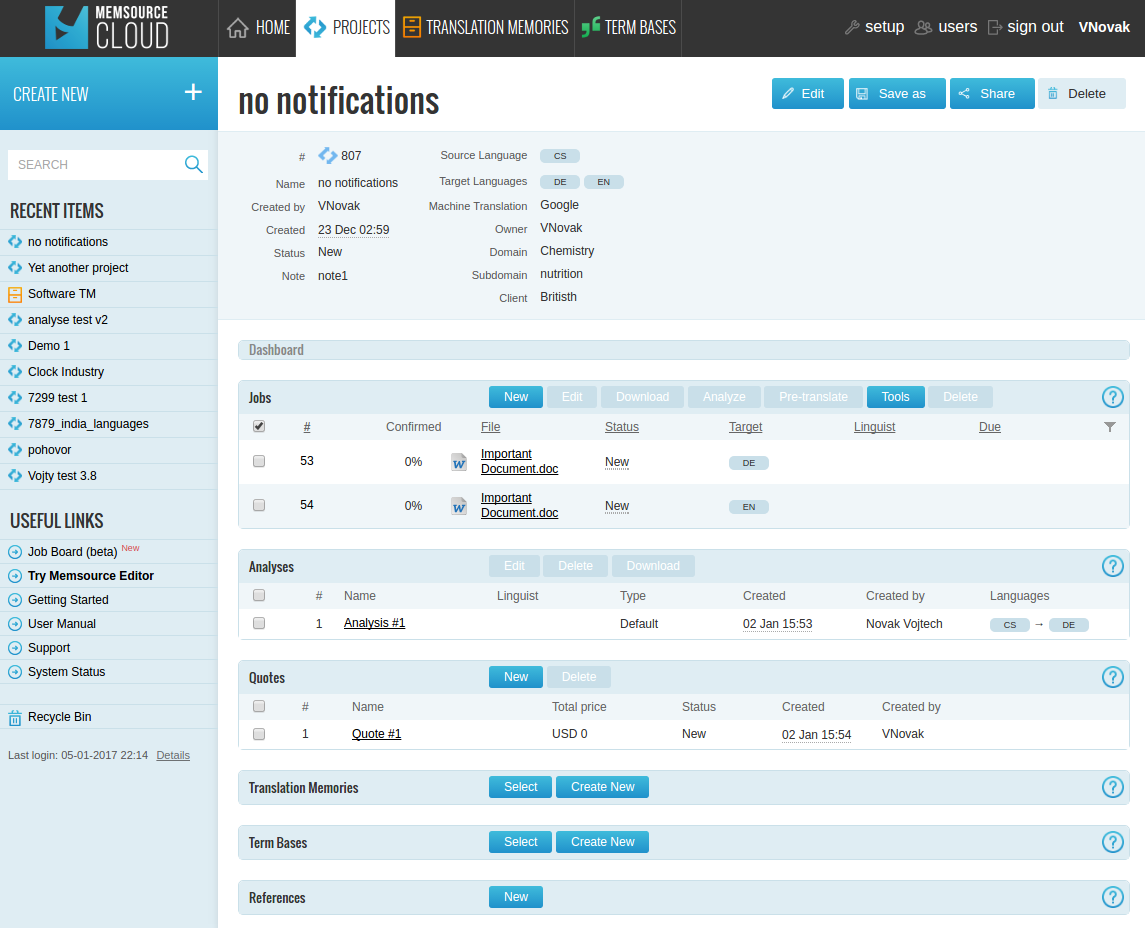
\includegraphics[width=1\textwidth]{pics/cloud/project}
	\caption{A translation project in Memsource Cloud}
	\label{fig:cloud}
\end{figure}

\section{Requirements}

The requirements for what the application has to support were determined gradually by a discussion with the Memsource developer team and CEO, followed by discussions with members of the support and product team who understand the customer use scenarios.
The outcome of conducted discussions is described in this section.

First I present a summary of requirements, a more detailed description is also included.

{\bf Summary of requirements}

Non-functional requirements
\begin{enumerate}
	\item app has to run on iOS and Android and be stable
	\item app should be written using technologies already used in Memsource
	\item UI components should have a platform-native look
	\item UI transitions have to feel smooth
	\item UI loading times not greater than 1.5 second on high-speed internet connections
	\item UI follows the design guidelines of both platforms
	\item app has to be intuitive to Memsource users
	\item app should keep number of API request minimal, to save resources
	\item the software has to be maintainable and testable
	\item use external software packages only if their license is suited for commercial use
\end{enumerate}

Functional requirements---the app has to:
\begin{enumerate}
	\item support Memsource project manager and translator roles
	\item support multiple users logged in at the same time and allow to switch between accounts
	\item list projects and allow to filter them
	\item list jobs and allow to filter them
	\item support adding jobs and projects
	\item allow to edit projects and jobs
	\item store user credentials in a secure manner
	\item support error reporting 
	\item use Memsource API to acquire the content
	\item present its UI in English only
\end{enumerate}

In some cases, the tools developed by Memsource are complex so that they support different user needs (for example lots of import options for translation jobs). We do not want to bring all this complexity to the mobile application and thus needed to find the features we wish the mobile app to include. 

The context in which the app will be used is a user needing to create, access or modify translation job and project information while being on the move or without access to a computer.

Follows a detailed description of requirements:


\begin{enumerate}
	\item User requirements
	\begin{enumerate}[label*=\arabic*.]
		\item The app will target handheld devices and a narrow group of users---professional users of Memsource Cloud who understand its features. 
		\item The app has to support the project manager and translator user roles 
		\begin{enumerate}[label*=\arabic*.]
			\item App has to support multiple users being logged into the app
			\item App will display content for only one user at a time and there will be a simple way to switch between users (i.e. set the active user).
			\item The number of added accounts will be limited to a maximum of four.
		\end{enumerate}
	\end{enumerate}
	
	The situation when a single Memsource user has several accounts is not common, but it is not unheard of (This does happen to users who work for several translation agencies). This will make working with several user accounts easier, without the need to log in and out or use several browser windows as is the case when using a computer. Currently, the API uses a token for authentication and this token is sent together with all requests. It is thus possible to make such requests for multiple users from the same device. Note that the API is available to only some of the Memsource editions.  
	
	\item Content requirements
	\begin{enumerate}[label*=\arabic*.]
		\item The app will load all its content through a public HTTP API which is provided by Memsource. In cases where a new API is needed, it will be developed.
		\item The app has to keep the number of API requests as low as possible so that the phone's and the servers' resources are not overused.
		\item The first screen should render within 4 seconds after starting the app.
	\end{enumerate}
	
	It follows that we assume the user will have internet connection available on their device at all times when the app is used to create new content and fetch the up-to-date data. 
	
	Compared to the web-based service, the app will only support selected features, to keep its UI simple and easy to work with. At the same time, it should follow the patterns users know from the web version to avoid confusion. More specifically: 
	
	\item Functionality requirements
	\begin{enumerate}[label*=\arabic*.]
		\item Functionality for PM users 
		
		\begin{enumerate}[label*=\arabic*.]
			\item The app has to support logging in for Memsource users whose role is project manager (PM).
			
			\item Project-related requirements
			\begin{enumerate}[label*=\arabic*.]
				\item App has to support listing projects based on their status (my projects, all, overdue, in progress). The list of projects should contain relevant information (name, customer, due date) for each project.
				\item App has to offer project search using the project name, when the project was created (last 24 hours, last 3 days, last 7 days, last 30 days), the client, the project owner and due date.
				\item PM has to be able to create a new project where they have to able to enter a predefined template from which project can be created, project name, client, domain and subdomain, business unit, source and target languages, due date and note.
				\item App will support deleting projects.
				\item App will support editing projects. The same project properties which are supported by the app when creating a new project will be supported for editing, with the addition of project owner.
				\item The app will allow the PM see project details (name, user who created the project, date when created, status, due date, source and target languages and project owner).
				\item App will support adding existing Translation memory and existing Term base to a project.
			\end{enumerate}
			
			\item Job-related requirements
			\begin{enumerate}[label*=\arabic*.]
				\item App will provide means to show a list of jobs contained in the project, showing relevant information for each job---job name, linguist name, due date, target languages and status.
				\item PM has to be able to create (upload) new translation jobs from document providers available on the platform.
				\item Adding jobs to project from an email attachment also has to be supported.
				\item When adding a new job, user will be able to enter the target languages, select due date, enter linguists for the job and have the option to notify them of the new job.
				\item After a job is uploaded, user has to be informed about it. Similarly, user has to be informed about unsuccessful file uploads.
				\item App should only support creating jobs from the most common file types (MS Word, Excel, Powerpoint and HTML).
				\item User needs to have the ability to select individual job, as well as several jobs, to download, edit and delete them. Editing consists of changing the linguist, status and due date.
				\item Similarly to searching and filtering of projects, the app will allow to filter jobs by name, status, target language, linguist and due date.
			\end{enumerate}
			%\item The application will not cover support for translating, i.e. Memsource Editor will not be a part of it since we found that it is overly complex to be used on a small screen of a mobile device.
			
		\end{enumerate}
		Note: The advanced project creation options for machine translation, analysis and other which are visible in Memsource Cloud, will not be included.
		
		\item Functionality for Linguist users
		\begin{enumerate}[label*=\arabic*.]
			\item The app will support listing projects that are visible to her, filtered based on status (new, accepted, completed). The list will contain relevant information---name, date created, owner, and source and target languages.
			\item User will be able to open a project, download or preview selected jobs and change their status (accepting or rejecting and marking them as completed). 
			\item Same as with a PM, translator will have the ability to search based on job filename, status, target languages and due date.
		\end{enumerate}
		
	\end{enumerate}
	
	
	
	\item Other requirements
	\begin{enumerate}[label*=\arabic*.]
		\item It is important the app be developed for at least the two major mobile phone platforms, that is Android and iOS.
		\item The app must be developed using programming languages that Memsource developers are already familiar with, that is one or more of: Java, Groovy, C++, JavaScript or any other technology if it brings substantial benefits.
		\item For the user, the app should look and feel as close to a native app as possible.
		\item The application has to support error reporting to allow Memsource continually improve the user experience, app stability and addition of new features.
	\end{enumerate}
	
\end{enumerate}
~


\section{Analysis of Platforms and Development Tools}

Today's market of mobile devices is largely divided between two platforms---iOS and Android. With 80.7\% for Android and 17.7\% for iOS, these two alone made up more than 98\% of worldwide sales in 4Q15, according to Gartner \cite{gartner}. Windows Phone comes third with 1.1\% of sales. Interestingly, in its March 2016 report, Kantar Worldpanel shows the sales of vary greatly among different states \cite{kantar}. For example, while iOS has a sales share of 56\% in Japan, it only has 17.8\% in Germany. As of Q1 2016, Android is growing in Europe, at the expense of iOS and Windows Phone, whose sales have been dropping in the UK and France where Windows Phone was historically relatively successful. The data from 3Q2016 shows growing Android sales: 86.8\%, 12.5\% and 0.3\% for Android, iOS and Windows Phone, respectively according to IDC \cite{idc:marketShare} and a report from Gartner \cite{gartner2} shows very similar numbers.


Since we are looking for a solution for creating apps for more than just one platform, I continue with describing the state of the art of multiplatform development tools.

\section{Xamarin}

Xamarin is a framework for developing native apps for iOS, Android and Windows Phone. The company was founded in 2011 and was acquired by Microsoft in 2016. All of Xamarin is now open-sourced on GitHub \footnote{https://github.com/xamarin}. 
Xamarin divides into four main parts: Xamarin.iOS, Xamarin.Android, Xamarin.Windows and Xamarin.Forms. The first three offer access to native APIs for the particular platforms, where Xamarin stresses that ``Anything you can do in Objective-C, Swift, or Java you can do in C\# with Xamarin'' \cite{xamarin:homepage} When using these, the developed solution consists of one project per supported platform (which contains the platform-specific code --- mainly the UI) plus single project whose code is shared and contains the business logic. Reportedly, this approach can result into about 75\% code reuse \cite{xamarin:codereuse}. Xamarin.Forms is an attempt to bring code reuse event higher, usually more than 90\% \cite{xamarin:codereuse} by sharing also the UI code.

As explained, UI in Xamarin can be either defined specifically for each platform within the platform's application project or cross-platform using Xamarin.Forms \cite{xamarin:forms}.

Taking the first way is recommended for apps with interactions that require native behavior, apps which use many platform-specific APIs or cases when custom-tailored UI has higher priority than code sharing. With this approach, each app will have its own UI defined in C\# code or XAML (an XML-like sytax for UI description) which can be done in a graphical UI designer.

Using Xamarin.Forms is best for apps that require little platform-specific functionality and apps where code sharing is more important than custom UI. Xamarin.Forms UI can be done either in C\# or in XAML but without the support of UI designer.

Development with Xamarin is done under Windows or OSX and the language of the framework is C\#. The code must be built and sent onto a device or emulator, which can take a considerable amount of time. Debugging is done in Visual Studio. Xamarin allows to write the code shared by all platforms in form of a Shared Project or a Portable Class Library \cite{xamarin:sharing_code} which are described in the following sections. 


\subsection{Shared Project}

Shared Project is the simplest way to share source code between platforms. This way, a cross-platform app that supports Android, iOS and Windows Phone would require an application project for each platform. Additionally, there would be a Shared Project for the code common to all projects.

The code within a Shared Project can be branched into platform-specific parts using compiler directives (e.g. using \#if \_\_ANDROID\_\_). The application projects can also include platform-specific references that the shared code can utilize.
The downside to this approach is that a Shared Project has no output assembly. During compilation, the files are treated as part of the referencing project and compiled into that project's DLL. This does not allow to distribute the code from Shared Project as an independent library.

\subsection{Portable Class Library}

Portable Class Library addresses the fact that Shared Project cannot be distributed as a standalone library. Portable Class Library offers the possibility to distribute it independently of the mobile app.

The disadvantages are that it is not possible to use compiler directives to reference platform-specific features and the fact that different platforms often use a different subset of the .NET Base Class Library (BCL) and therefore only such subset is available to use. This, however, can be to some extent circumvented by the Provider pattern or Dependency Injection. That way, the actual implementation is coded in the platform projects against an interface defined within the Portable Class Library.


\section{React Native}

React Native (RN) is a counterpart of the popular web development library React and is also developed by Facebook which uses in several production apps and ``will continue to invest in it'' \footnote{https://facebook.github.io/react-native}. It was first released in 2015, which makes it the youngest among the covered solutions. React is popularized under the slogan ``Learn once, write anywhere.'', as opposed to e.g. Java whose goal is that one codebase runs anywhere, this means that once a developer learns React, she can use her skills to write apps for multiple platforms (web, Android, iOS, etc.) using just React, but not necessarily with a single codebase.

React originally started as a tool for describing user interfaces for the web, and rapidly became popular within the web development community. However, it was recognized that React's usage was not limited only to web.

React describes the user interface through reusable components which tell what the UI is supposed to look like. It is then the matter of transforming the description into a user-facing UI. On the web, this is the task of React-DOM which uses the Virtual DOM tree as a layer of abstraction between the developer's code and what is rendered in the browser. When programming mobile apps, this abstraction is handled by React Native. At this point, it is important to state that the UI rendered with React Native is not running in a WebView but is built from the native UI elements of the platform in question (i.e. \texttt{View} on Android and \texttt{UIView} on iOS), which makes it different from the longer-established hybrid development environments which also use JavaScript. 

RN application code is written in JavaScript which runs in JavaScriptCore engine on the device \cite{rn:jsenviroment}. RN features what is called a \textit{bridge} \cite{rn:bridge}. The bridge is in turn responsible for bridging the calls onto the native platform APIs and back. This way, user can access any native functionality and get information back in a callback or promise payload.

When developing with RN, the developer creates or makes use of ready-made UI components and uses them to compose the application UI. The components are written in a combination of JavaScript and XML tags, called JSX. Optionally, Flow \footnote{http://flowtype.org/}, a static type checker for JavaScript can be used. Also supported although not so frequently used are languages that transpile to JavaScript, such as TypeScript \footnote{https://www.typescriptlang.org/}. From developer's point of view, important features of RN are its live and hot reloading \cite{rn:hotreload}. Live reloading \index{live reloading} enables the developer to apply code changes to the app running on a device or in an emulator quickly. Live reload in fact takes about five seconds on my development machine. This is a tremendous improvement over traditional native development, which until recently---with the introduction of Instant Run into Android Studio---suffered from the slow process of building an app and loading it into a device or emulator.

The other feature called Hot Reloading \index{hot reloading} offers essentially the same functionality as Live Reloading with the advantage of being faster and preserving the application state---the screen displayed before and after the Hot Reload is the same---thanks to which the developer does not need to navigate through the app to the screen where the change is being done. This is especially helpful for making changes to the UI layout and styles because Hot Reload needs about one second to take effect. These features can significantly accelerate app development and improve the developer experience. The downside of Hot Reloading is that it mostly works for simple changes in the UI but fails when modifications are of larger extent.

Debugging RN is accomplished through running the code in Chrome browser or external debugging tools (such as those included with Visual Studio Code or Webstorm) where user can set breakpoints and work with code similarly to working in web development. In this case, all the JavaScript code runs within Chrome's V8 engine itself and communicates with the phone or emulator via WebSockets.


\subsection{Native Modules}

When a developer needs native functionality which is not already provided by RN, they will often find such functionality already implemented by the community which surrounds RN. In such case, the component is available through the Node package manager (npm).

In case the functionality is not yet implemented, the developer can create a native module \index{native module} \cite{rn:nativemodules} for it. Native module consists of code written in Java (for Android) and Objective-C (or Swift) for iOS which implements the desired functionality and of JavaScript code that will expose the native functionality to the app's JavaScript code. The native code is invoked from JavaScript through the RN bridge and results (if any) can be passed back by a Promise or callback. Native modules give developer the freedom to implement any functionality desired, as long as it is available on the platform, but have the downside of needing to code both for iOS and Android in the language of the platform.


% pridani do indexu: \emph{affine}\index{affine}
\section{Ionic}

In version 2.RC4 as of 1/2017, Ionic \footnote{http://ionicframework.com} is another successful framework for developing cross-platform mobile apps which was initially released in 2013. Ionic is a hybrid framework, meaning an app created with it runs in a WebView, same as a website would---with the important difference that it can also use the native device APIs. It supports iOS, Android and Windows Phone.

Just like the aforementioned frameworks, Ionic is open source and offers a set of mobile-optimized components written in HTML, CSS and JavaScript. Ionic 2 is integrates with Angular 2, a framework for web development from Google. Ionic has put o lot of work into providing components that are styled according to each supported platform, thus saving the developer's time by not having to spend valuable time by styling the UI. Compared to React Native and Xamarin, Ionic gives less flexibility in customizing the app for different platform. With Xamarin and RN, developer can make the app look and behave completely different (at the expense of writing more code) while this is limited on Ionic. Depending on the particular app context, this can be both a downside or a benefit.

Ionic 2 developer can optionally choose to develop in TypeScript, which is a language that compiles to plain JavaScript. As its name reveals, the most important TypeScript's feature is addition of types to JavaScript. This can reveal errors before they happen, and gives extra information to both the developer and IDE (Integrated Development Environment) which therefore can offer better code completion. TypeScript is basically a competitor of Flow.

Ionic runs inside Apache Cordova, a mobile application development framework which provides access to native platform features such as camera, sensors, filesystem or contacts. Access to arbitrary features can be allowed through plugins, which are composed of a single JavaScript interface used on all platforms, and platform-specific code code which is called from JavaScript. In this respect, Cordova Plugins are similar to native modules in RN.

Ionic does more than only mobile app development. It offers features like ionic lab, which allows to run iOS and Android apps one next to the other in browser as well as in a GUI application for Windows and Mac. There is also the Ionic Market, which contains lots of starter templates and themes. Ionic's View app allows developer to easily share apps with customers and testers. Ionic Creator is a prototyping tool where developer can drag and drop components to create a simple app an even export it as an Ionic app.

Also, with live reloading, the iteration process is a lot faster than traditional procedures involving compilation.


\section{Conclusions}

There is currently a very strong competition in the area of multiplatform mobile app frameworks and choosing the right one for one's needs is difficult. All of the researched solutions are very capable. 
After developing simple proof-of-concept apps using the three described frameworks I first ruled out Xamarin. Although C\# can be considered a very mature and powerful language, the reasons for ruling Xamarin out were the need to write UI twice - which would involve learning the specifics of Android as well as iOS. We did not want to use Xamarin.Forms because we were uncertain about whether it would not limit us and the available demonstrations apps written using Xamarin.Forms did not make a very good impression on me (the official Xamarin Evolve conference app took long to start and froze several times my Nexus phone). Moreover, Xamarin's slow development iteration cycle, for me, felt like a big drawback.

Ionic 2 is a popular framework. After creating simple application in it, I could not help but notice very slow startup times: between 6 and 9 seconds for a very simple app. This issue was confirmed by posts in the community forum and according to an Ionic representative, the startup time will be improved. Moreover, after installing several apps developed in Ionic we noticed not all of them work on all devices (probably due to cpu family), which left me with mixed feelings. The advantage of Ionic 2 surely lays in its maturity, strong community and lots of readymade UI widgets styled differently for each platform.

React Native was chosen after difficult comparisons. Its advantages are that it is backed and used by Facebook, it is being developed at a quick pace and has a growing community with lots of components available or in development. It also provides greater UI flexibility than Ionic, better performance, and the ability to easily communicate with native code is a need for our use case since the app will have to deal a lot with files (background file uploads, downloads, opening the app with them). Most importantly, RN does a very good job at transforming the React code to the native views. Obvious disadvantage is its immaturity and probably the need to work harder to get eye-appealing designs because unlike Ionic, RN does not offer styled UI components ready to be used but only the essential components with no multiplatform styling. 

Table \ref{tab:comparison} provides a quick comparison of the described libraries or frameworks against selected criteria. Plus sign (+) denotes positive rating, while zero (0) and minus (-) denote neutral and negative rating.

\begin{table}[htbp]
	\centering
	\caption{Comparison of the considered multiplatform development tools}
	\label{tab:comparison}
	\renewcommand{\arraystretch}{1.2}
	\begin{ctucolortab}
	\begin{tabularx}{\textwidth}{XYYYY}

		\textbf{Platform} & \textbf{Xamarin} & \textbf{Xamarin Forms} & \textbf{Ionic 2} & \textbf{React Native}\\ \hline
development speed          & -                           & -                                 & +                           & +                                \\ \hline
performance                & +                           & +                                 & -                           & 0                                \\ \hline
maturity              & +                           & 0                                 & +                           & -           \\ \hline
platform-specific behavior & +                           & -                                 & -                           & +                                
      
	\end{tabularx}%
\end{ctucolortab}
\end{table}%


